\begin{figure}[!h]
	\centering
	\subbottom[aerial image as input\label{fig:defgeoseg1}]{
		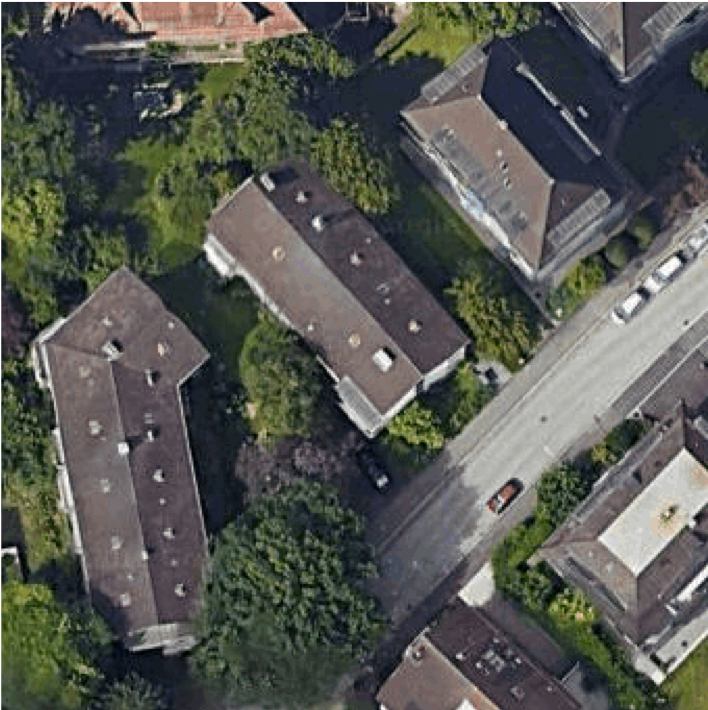
\includegraphics[width=\figfig\textwidth]{1-03-0.png}
	}
	\subbottom[expected polygons as output\label{fig:defgeoseg2}]{
		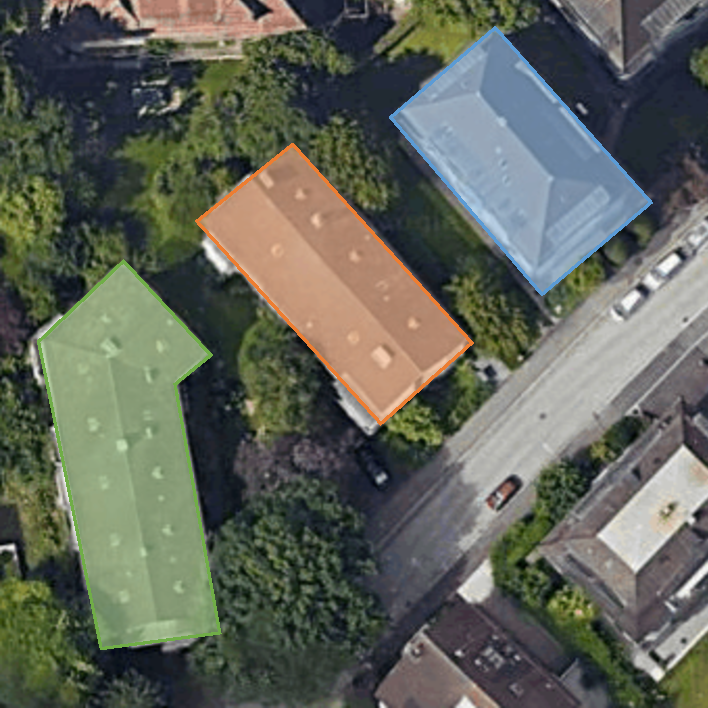
\includegraphics[width=\figfig\textwidth]{1-03-1.pdf}
	}
    \caption[Example of instance segmentation of geometrical shapes in an aerial image]{Example of instance segmentation of geometrical shapes in an aerial image. (a) is the input aerial image containing 3 complete buildings. (b) is the visualized result for output polygons.}
	\label{fig:defgeoseg}
\end{figure}